\subsection{Detection Performance Evaluation}

\subsubsection{Quantitative Evaluation Results}

The detection performance of the two models on the validation set is summarized in Table~\ref{tab:detection_results}. Following the default YOLOv8 model selection strategy, the best checkpoint is selected according to a weighted fitness metric:
\[
\mathrm{fitness} = 0.1 \cdot \mathrm{mAP}_{50} + 0.9 \cdot \mathrm{mAP}_{50\text{-}95}.
\]
This strategy places greater emphasis on localization quality under stricter IoU thresholds.

\begin{table}[H]
    \centering
    \caption{Detection performance comparison on the VisDrone validation set.}
    \label{tab:detection_results}
    \begin{tabular}{lcccc}
        \toprule
        Configuration & mAP@50 & mAP@50:95 & Precision & Recall \\
        \midrule
        YOLOv8n-$640$ & 32\% & 18\% & 45\% & 34\% \\
        YOLOv8s-$768$ & 44\% & 26\% & 57\% & 44\% \\
        \bottomrule
    \end{tabular}
\end{table}

Compared with YOLOv8n-$640$, YOLOv8s-$768$ improves mAP@50 from 32\% to 44\% and mAP@50:95 from 18\% to 26\%. According to Table~\ref{tab:yolov8_configs}, the computational cost increases from 8.204 GFLOPS to 28.666 GFLOPS, corresponding to an approximately 3.5$\times$ increase in computation. Meanwhile, the actual PyTorch single-image inference latency increases from 1.309 ms to 2.962 ms.

Despite the increased computational cost, the larger model and higher input resolution provide substantial improvements in detection performance. This result suggests that, within the memory constraints of the target edge hardware platform, jointly scaling model capacity and input resolution is an effective strategy for improving small-object detection performance on the VisDrone dataset.

Figure~\ref{fig:map_curves} compares the validation mAP curves of the two models during training. YOLOv8s-$768$ consistently outperforms YOLOv8n-$640$ throughout training. Notably, YOLOv8s-$768$ surpasses the best mAP achieved by YOLOv8n-$640$ within only a few epochs, indicating significantly stronger feature representation capability for dense aerial object detection.

\begin{figure}[H]
    \centering
    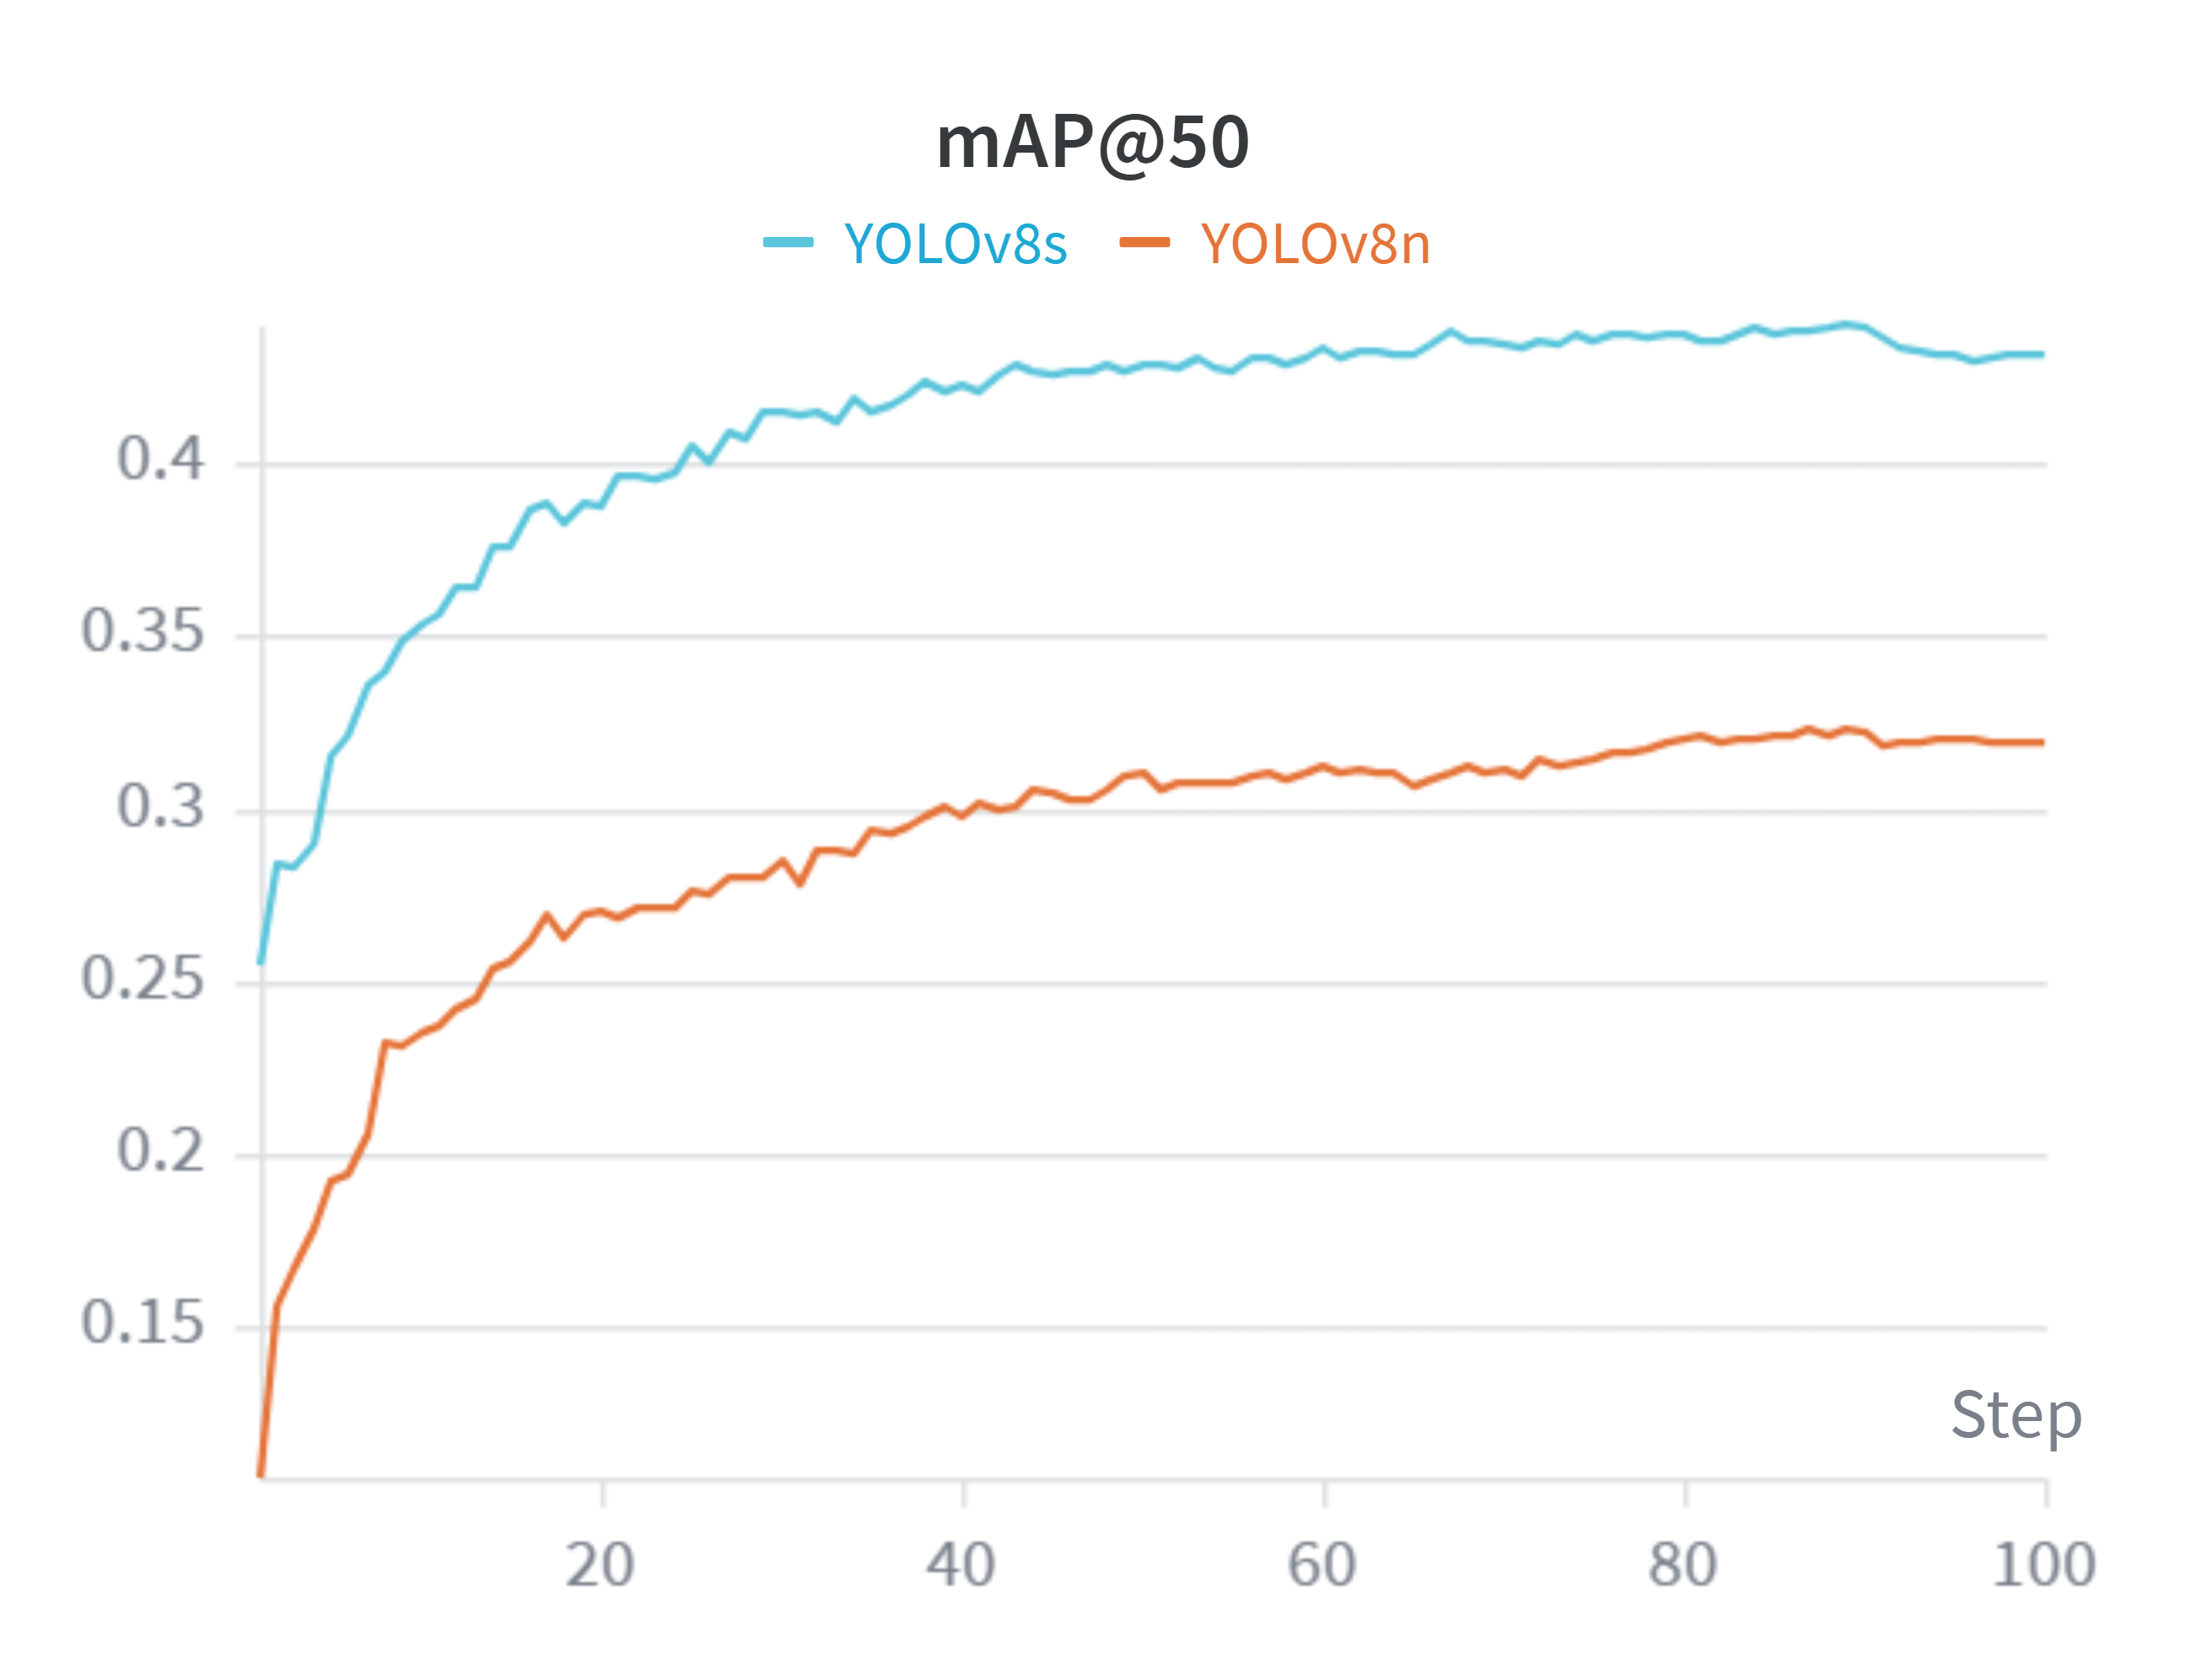
\includegraphics[width=0.45\textwidth]{figures/task2/mAP@50.png}
    \hfill
    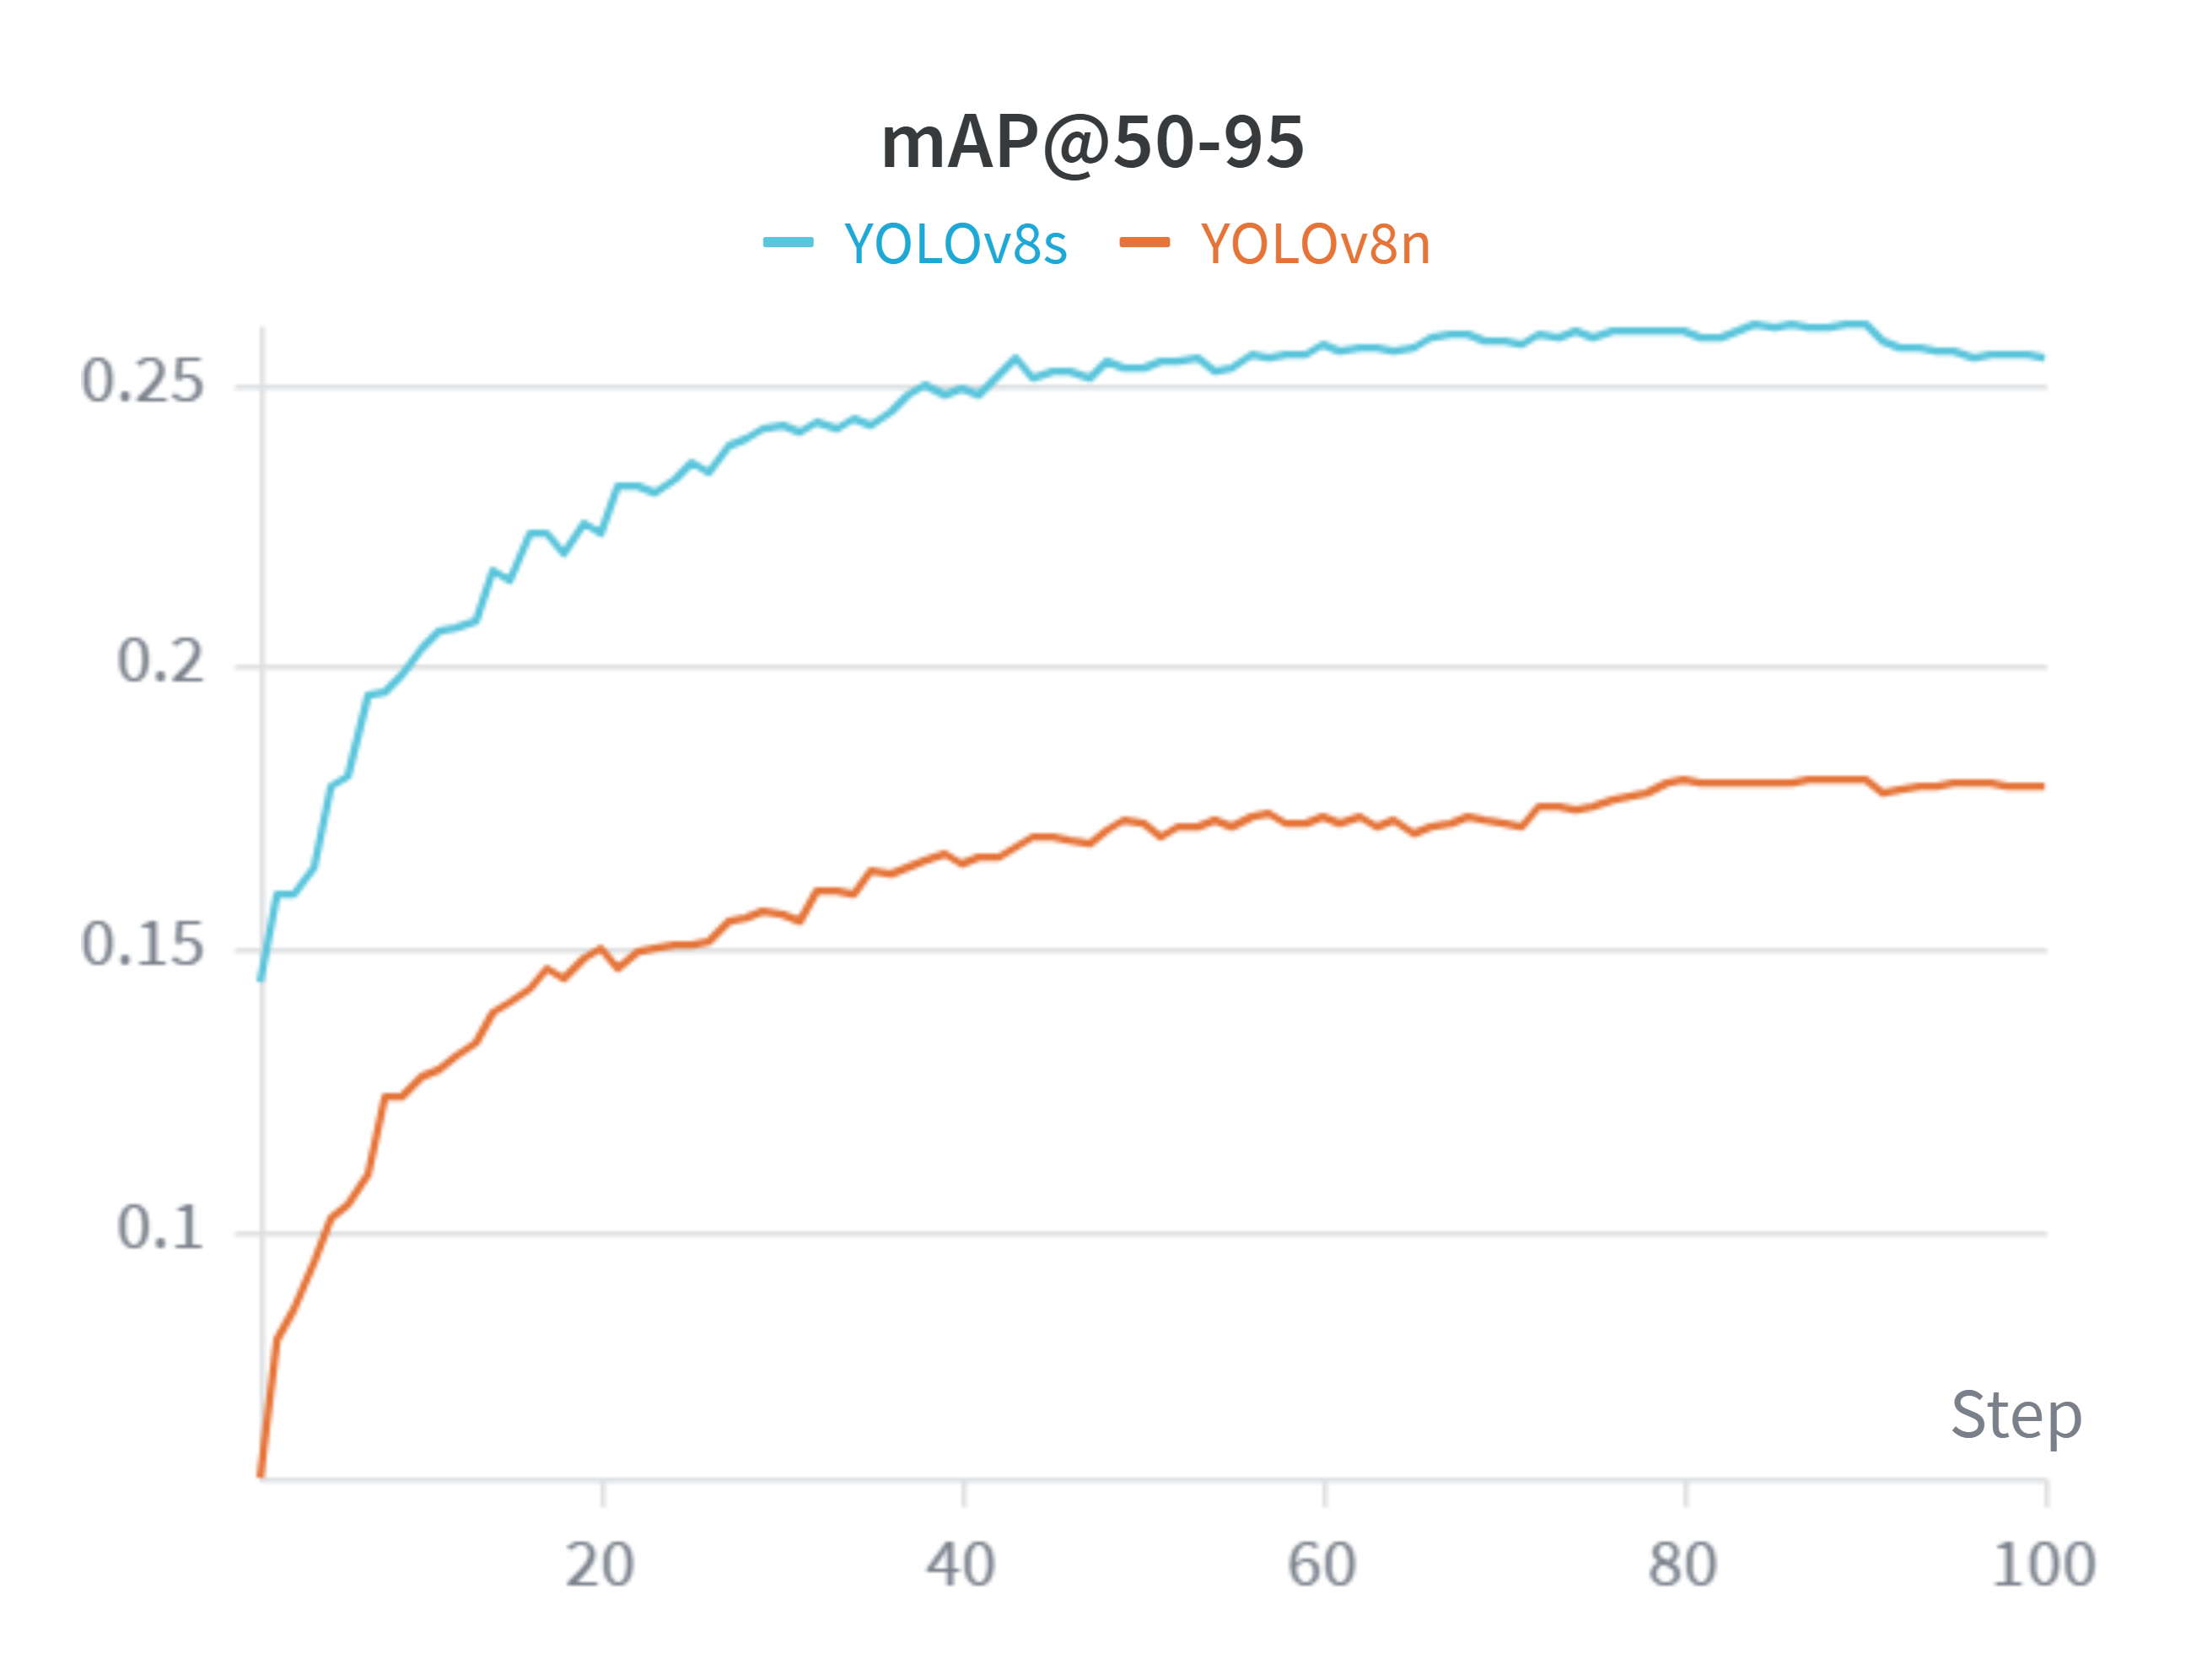
\includegraphics[width=0.45\textwidth]{figures/task2/mAP@50-95.png}
    \caption{Comparison of validation mAP curves during training.}
    \label{fig:map_curves}
\end{figure}

\subsubsection{Precision--Recall and Confidence Analysis}

Figure~\ref{fig:pr_curve} shows the Precision--Recall curves of the two models for different object categories. For every category, the curves of YOLOv8s-$768$ are consistently closer to the upper-right corner, indicating better precision-recall trade-offs and larger Average Precision (AP) values across all classes.

\begin{figure}[H]
    \centering
    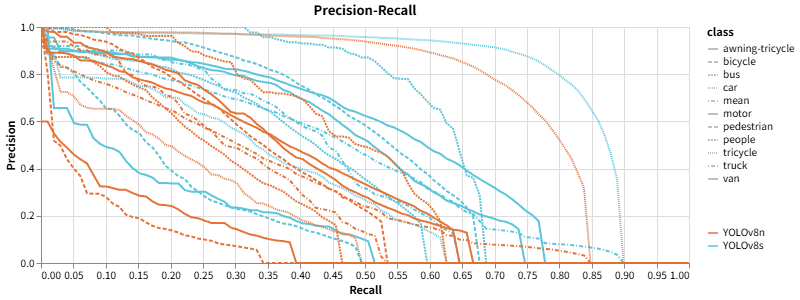
\includegraphics[width=0.75\textwidth]{figures/task2/Precision Recall.png}
    \caption{Precision--Recall curves of different object categories.}
    \label{fig:pr_curve}
\end{figure}

Figure~\ref{fig:f1_curve} shows the relationship between F1 score and confidence threshold on the validation set. Different object categories exhibit noticeably different optimal confidence intervals. Some difficult categories achieve their highest F1 scores at relatively low confidence thresholds (approximately 0.14), while easier categories perform better at higher thresholds (approximately 0.37).

To balance multi-class performance while maintaining deployment simplicity, the final system adopts the peak point of the global averaged F1 curve as the unified inference threshold:
\[
\texttt{conf\_thres} = 0.25.
\]
In practice, category-specific confidence thresholds could also be adopted to further improve detection performance for particular object classes if required.

\begin{figure}[H]
    \centering
    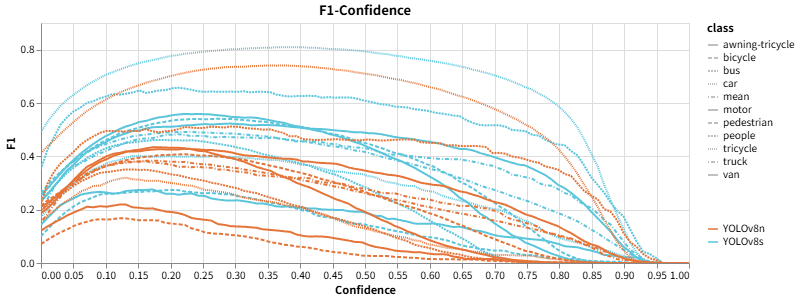
\includegraphics[width=0.75\textwidth]{figures/task2/F1 Confidence.png}
    \caption{Relationship between F1 score and confidence threshold.}
    \label{fig:f1_curve}
\end{figure}
